\subsection{Simulator}

In diesem Kapitel wird das Erarbeiten des Konzeptes des Simulators, der Implementierung und der Resultate festgehalten. Das Ziel des Simulators ist es, die Navigation und denn Ablauf des Roboters bei der Traversierung des Graphes zu simulieren.


\subsubsection{Spezifikationen}

Die Spezifikationen aufgelistet in Tabelle \ref{table:spezifikation-simulator} soll der Simulator erfüllen.

\begin{table}[H]
\centering
\small
\begin{tabularx}{\textwidth}{|l|X|l|}
\hline
  \textbf{Nr.} & \textbf{Spezifikation} & \textbf{Priorität 1-3}  \\
  \hline
  1  & Der Zielknoten kann ausgewählt werden. &  2\\
  \hline
   2   & Der Roboter speichert den Graph intern.  & 1\\
  \hline
   3 & Der Roboter überprüft seine Nachbarsknoten.&1\\
  \hline
  4 & Der Roboter erkennt fehlende Linien und reagiert darauf. & 1\\
  \hline
  5 &   Der Roboter erkennt Pylonen und reagiert darauf. & 1\\
  \hline
   6  &   Der Roboter erkennt Barrieren und reagiert darauf. & 1\\
  \hline
    7 &   Der Roboter berechnet den kürzesten Weg im Graphen.& 1\\
  \hline
     8  &   Der Weg des Roboters wird im GUI angezeigt. & 1\\
  \hline
      9   &   Die Reaktionen auf die Hindernisse werden im GUI angezeigt. & 3\\
  \hline
 10   &   Die Hindernisse werden im GUI angezeigt. & 2\\
  \hline
   11   &   Es lassen sich zufällige Graphen mit zufällig platzierten Hindernissen erstellen. & 2\\
  \hline
   12   &   Die Geschwindigkeit des Roboters lässt sich einstellen. & 2\\
  \hline
   13   &   Die Traversierung des Graphens durch den Roboter kann automatisiert simuliert werden. & 2\\
  \hline

\end{tabularx}
\caption{Spezifikationen Simulator}
\label{table:spezifikation-simulator}
\end{table}

\subsubsection{Konzeption}

Mit einem morphologischen Kasten (siehe Anhang \nameref{mk-simulator}) wurden mehrere Varianten ermittelt, die alle die Spezifikationen erfüllen können. Mit einer Nutzwertanalyse (siehe Anhang \nameref{nutzwertanalyse}) wurde die beste Variante bestimmt:

\begin{itemize}
    \item Programmiersprache: Python
    \item Wegnetz einlesen: \gls{yaml}
    \item Wegnetz intern speichern: Key-Values
    \item Bewegliche Hindernisse erfassen: Gewichtung
    \item Blockierte Knoten erfassen: Knoten entfernen
    \item Wegfindung: eigene Implementation
    \item Clientseitige Kommunikation \acrshort{i/o}: \acrshort{gui}
\end{itemize}

Die einzelnen Tätigkeiten werden in GitHub Issues festgehalten. Die einzelnen Features wurden unter den Entwickelnden aufgeteilt und via GitHub Issues assigned. So ist sichtbar, wer woran arbeitet.

\begin{figure}[H]
\centering
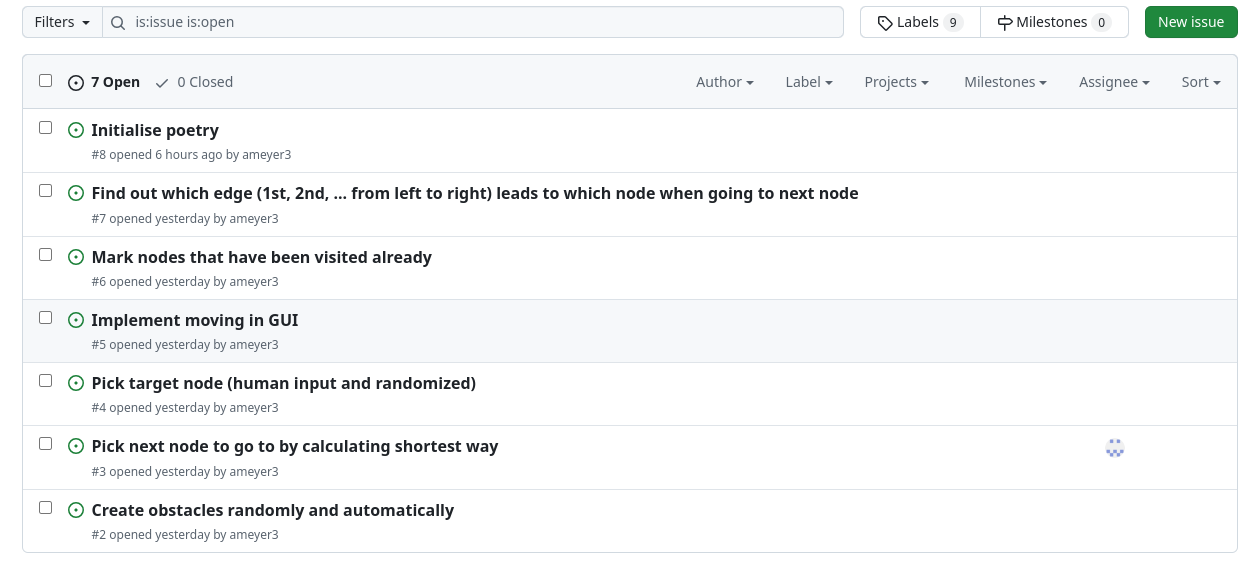
\includegraphics[width=\textwidth]{img/github-issues.png}
\caption{Ausschnitt GitHub Issue Liste}
\label{fig:github-issues}
\end{figure}

Das Klassendiagramm des Simulators wurde zum Verständnis in zwei Diagramme aufgeteilt. Im ersten Diagramm sind die Klassen aufgezeigt, die auch in dem richtigen Roboter wieder verwendet werden. Das zweite Diagramm detailliert diese Klassen, die nur für den Simulator erstellt wurden.

Es wurde ein objektorientierter Ansatz gewählt, um den Simulator umzusetzen. Die Roboter-Klasse soll dabei den physischen Roboter darstellen, der die einzelnen Bauteile besitzt. So soll zum Beispiel die Wheels-Klasse als Simulation für das Drehen und Fortbewegen dienen. An diese Klasse werden die Nachrichten gesendet, welche im echten Roboter an die elektrische Steuerung des Motors gesendet werden würden.

In Abbildung \ref{fig:simulator-classdia-robot} sind die Roboterklassen dargestellt. Der GraphHandler wird verwendet, um den Graph intern zu speichern und auszulesen. Der Path Calculator berechnet den kürzesten Weg zum Zielknoten mit einem \gls{dijkstra} Algorithmus.

Es gibt zusätzlich zum normalen Modus (\verb|run_normal_mode|) auch einen Modus, in dem der Roboter sich blind durch den Graphen bewegt, falls dieser nicht mehr weiss, wo er sich befindet (\verb|run_blind_testing_mode|). Dieser wird im folgenden Abschnitt ``Trial and Error'' noch weiter erklärt. Im Klassendiagramm sind die Methoden im Roboter so dargestellt, dass diese Methoden, die nur für einen bestimmten Modus verwendet werden, direkt unterhalb der öffentlichen \verb|run| Methoden ist. Diese Methoden, die sich zuunterst befinden, werden von allen Modi verwendet. 

\begin{figure}[H]
\centering
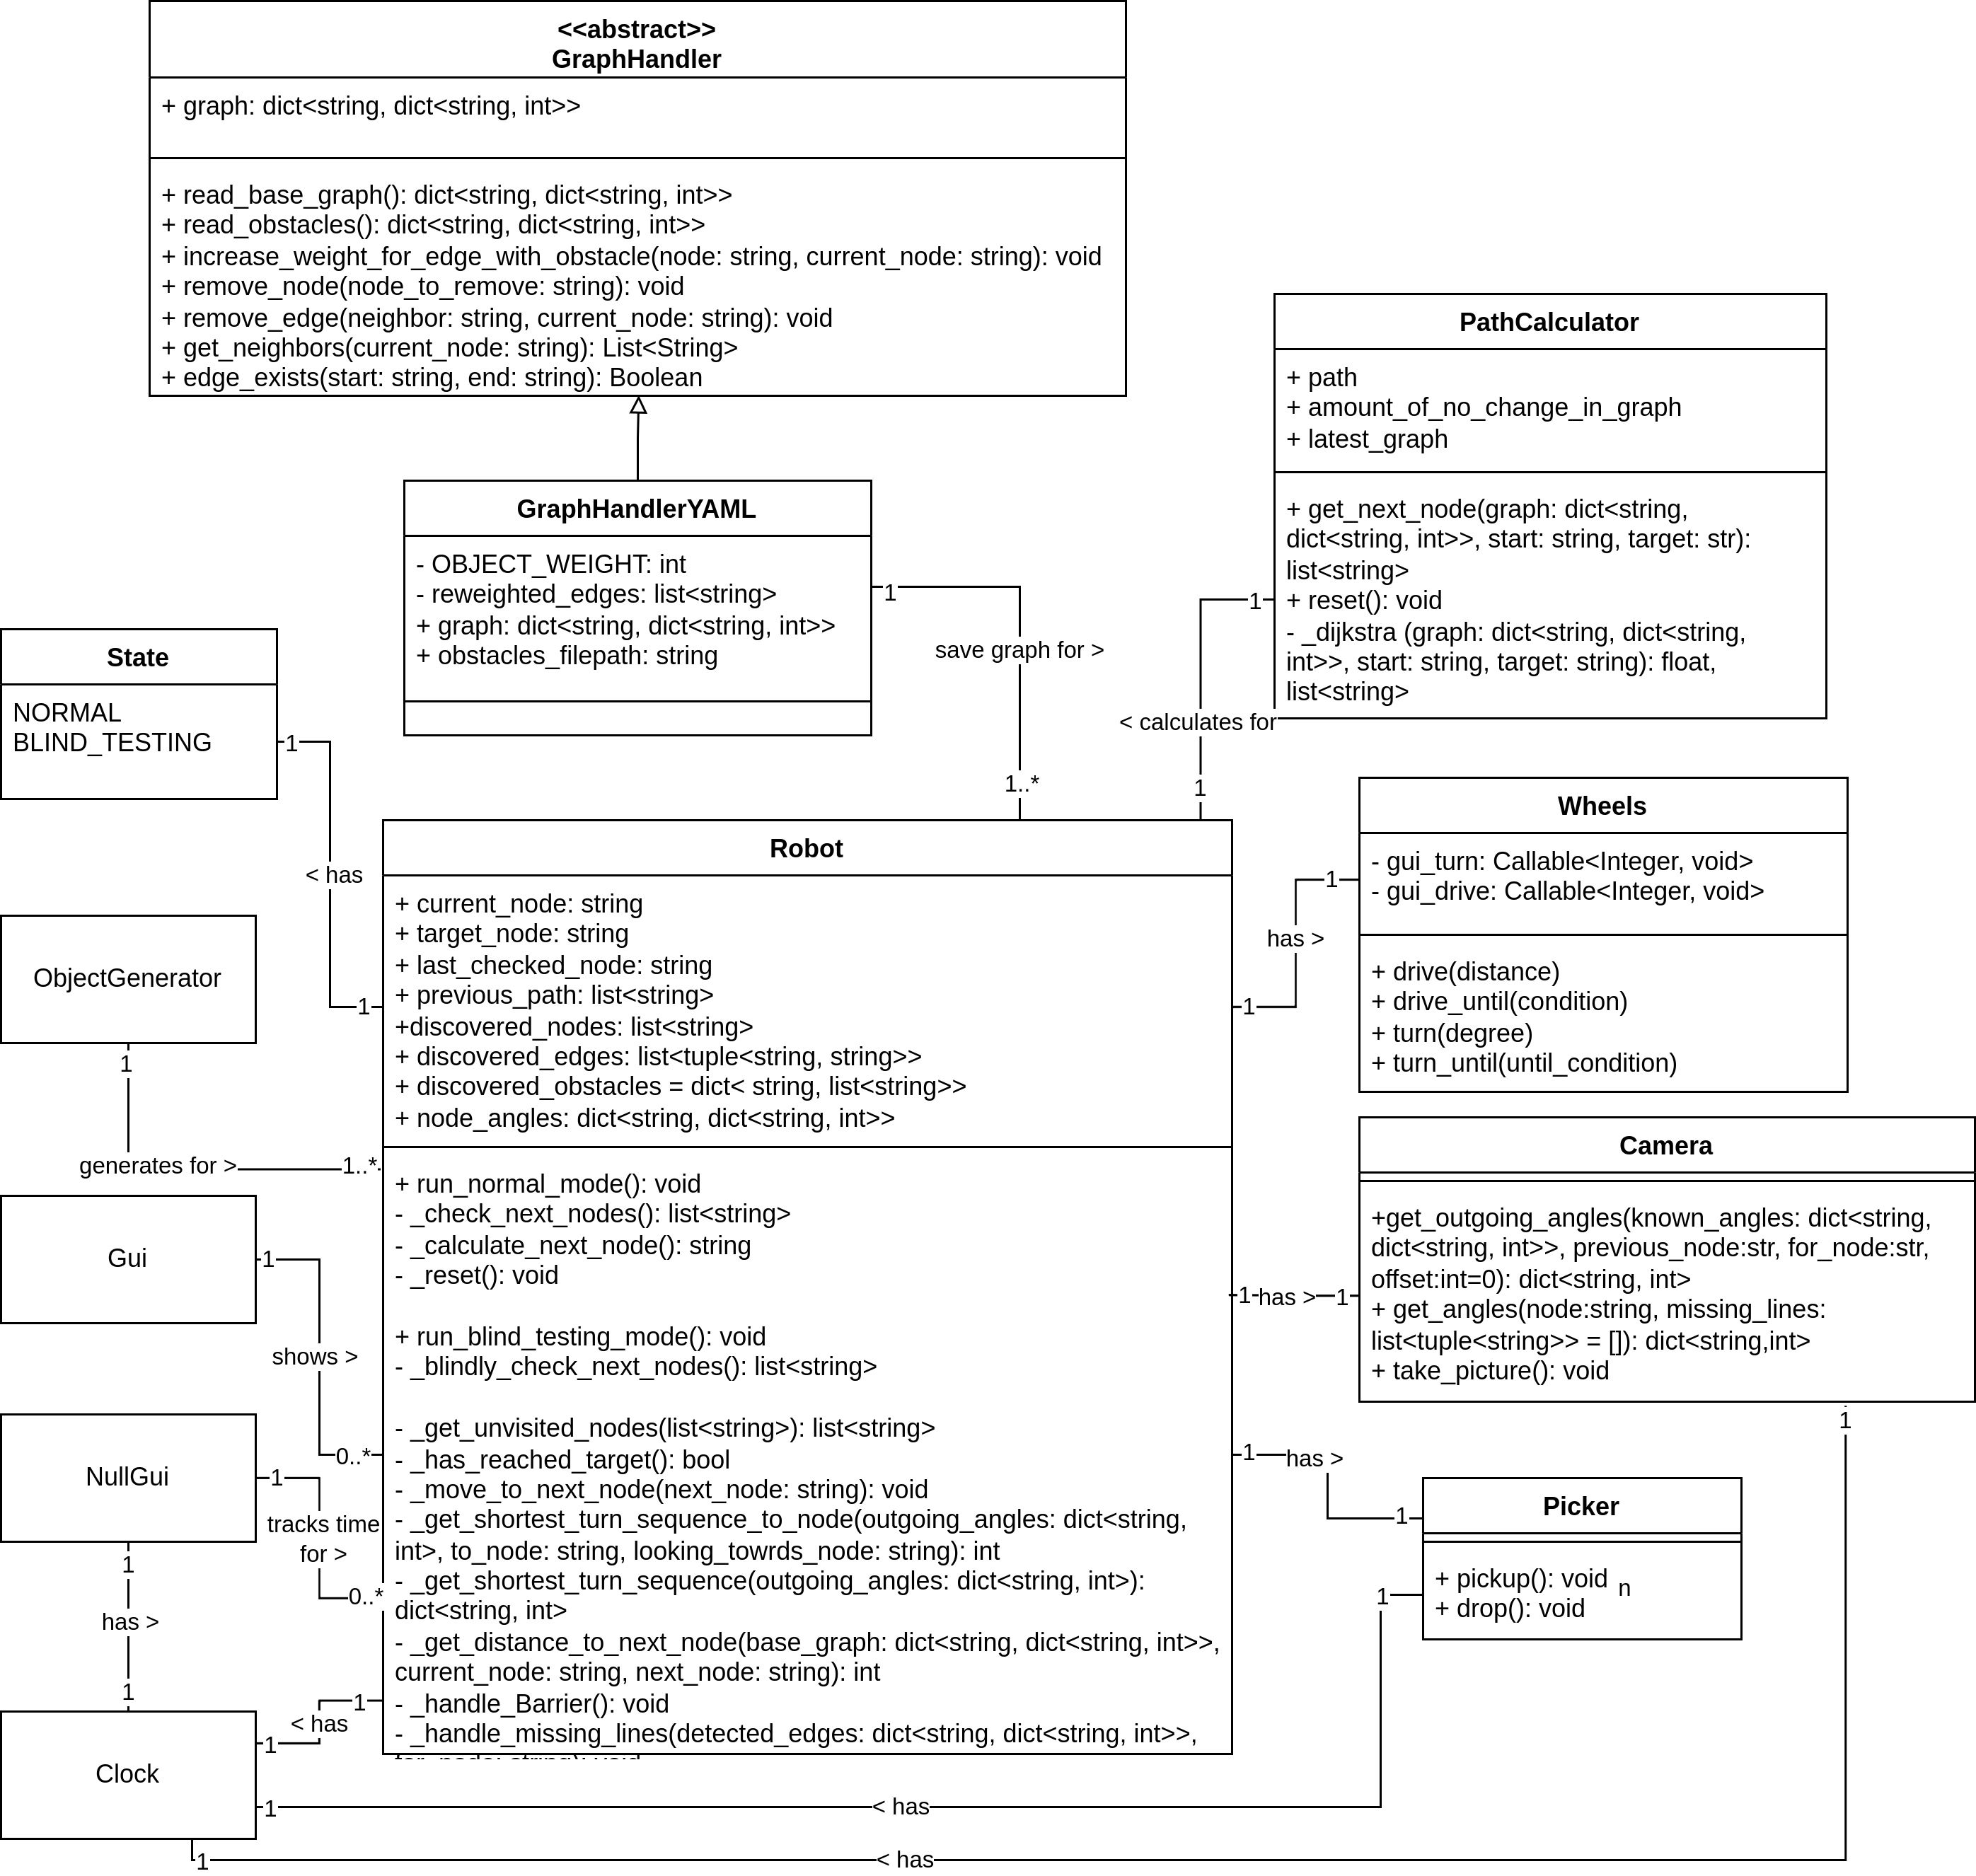
\includegraphics[width=\textwidth]{assets/informatik-prototyp/simulator/simulator-robot-erd.png}
\caption{Simulator Klassendiagramm: Roboter Klassen}
\label{fig:simulator-classdia-robot}
\end{figure}

Auf der Abbildung \ref{fig:simulator-classdia-sim} sind die Klassen ausgeführt, die nur für den Simulator benötigt werden und nicht für den Roboter. Das \acrshort{gui} zeigt den Graphen und die Fahrt des Roboters, dies ist im Abschnitt \ref{gui} gezeigt. Die Clock Klasse zählt die Zeit, die der Roboter für einzelne Aktivitäten benötigt. Das NullGUI hat kein User Interface, zählt jedoch die Zeit, die der Roboter für die einzelnen Fahrten benötigt. Mit dem NullGUI können viele Fahrten schnell simuliert werden. Dies ermöglicht eine akkurate Zeitmessung, obwohl die Traversierung und die Simulation beschleunigt sind. Der ObstacleGenerator erstellt automatisch mögliche Graphenkonfigurationen. Damit können verschiedene Graphen simuliert und nachfolgend befahren werden, um das Konzept zu testen.

\begin{figure}[H]
\centering
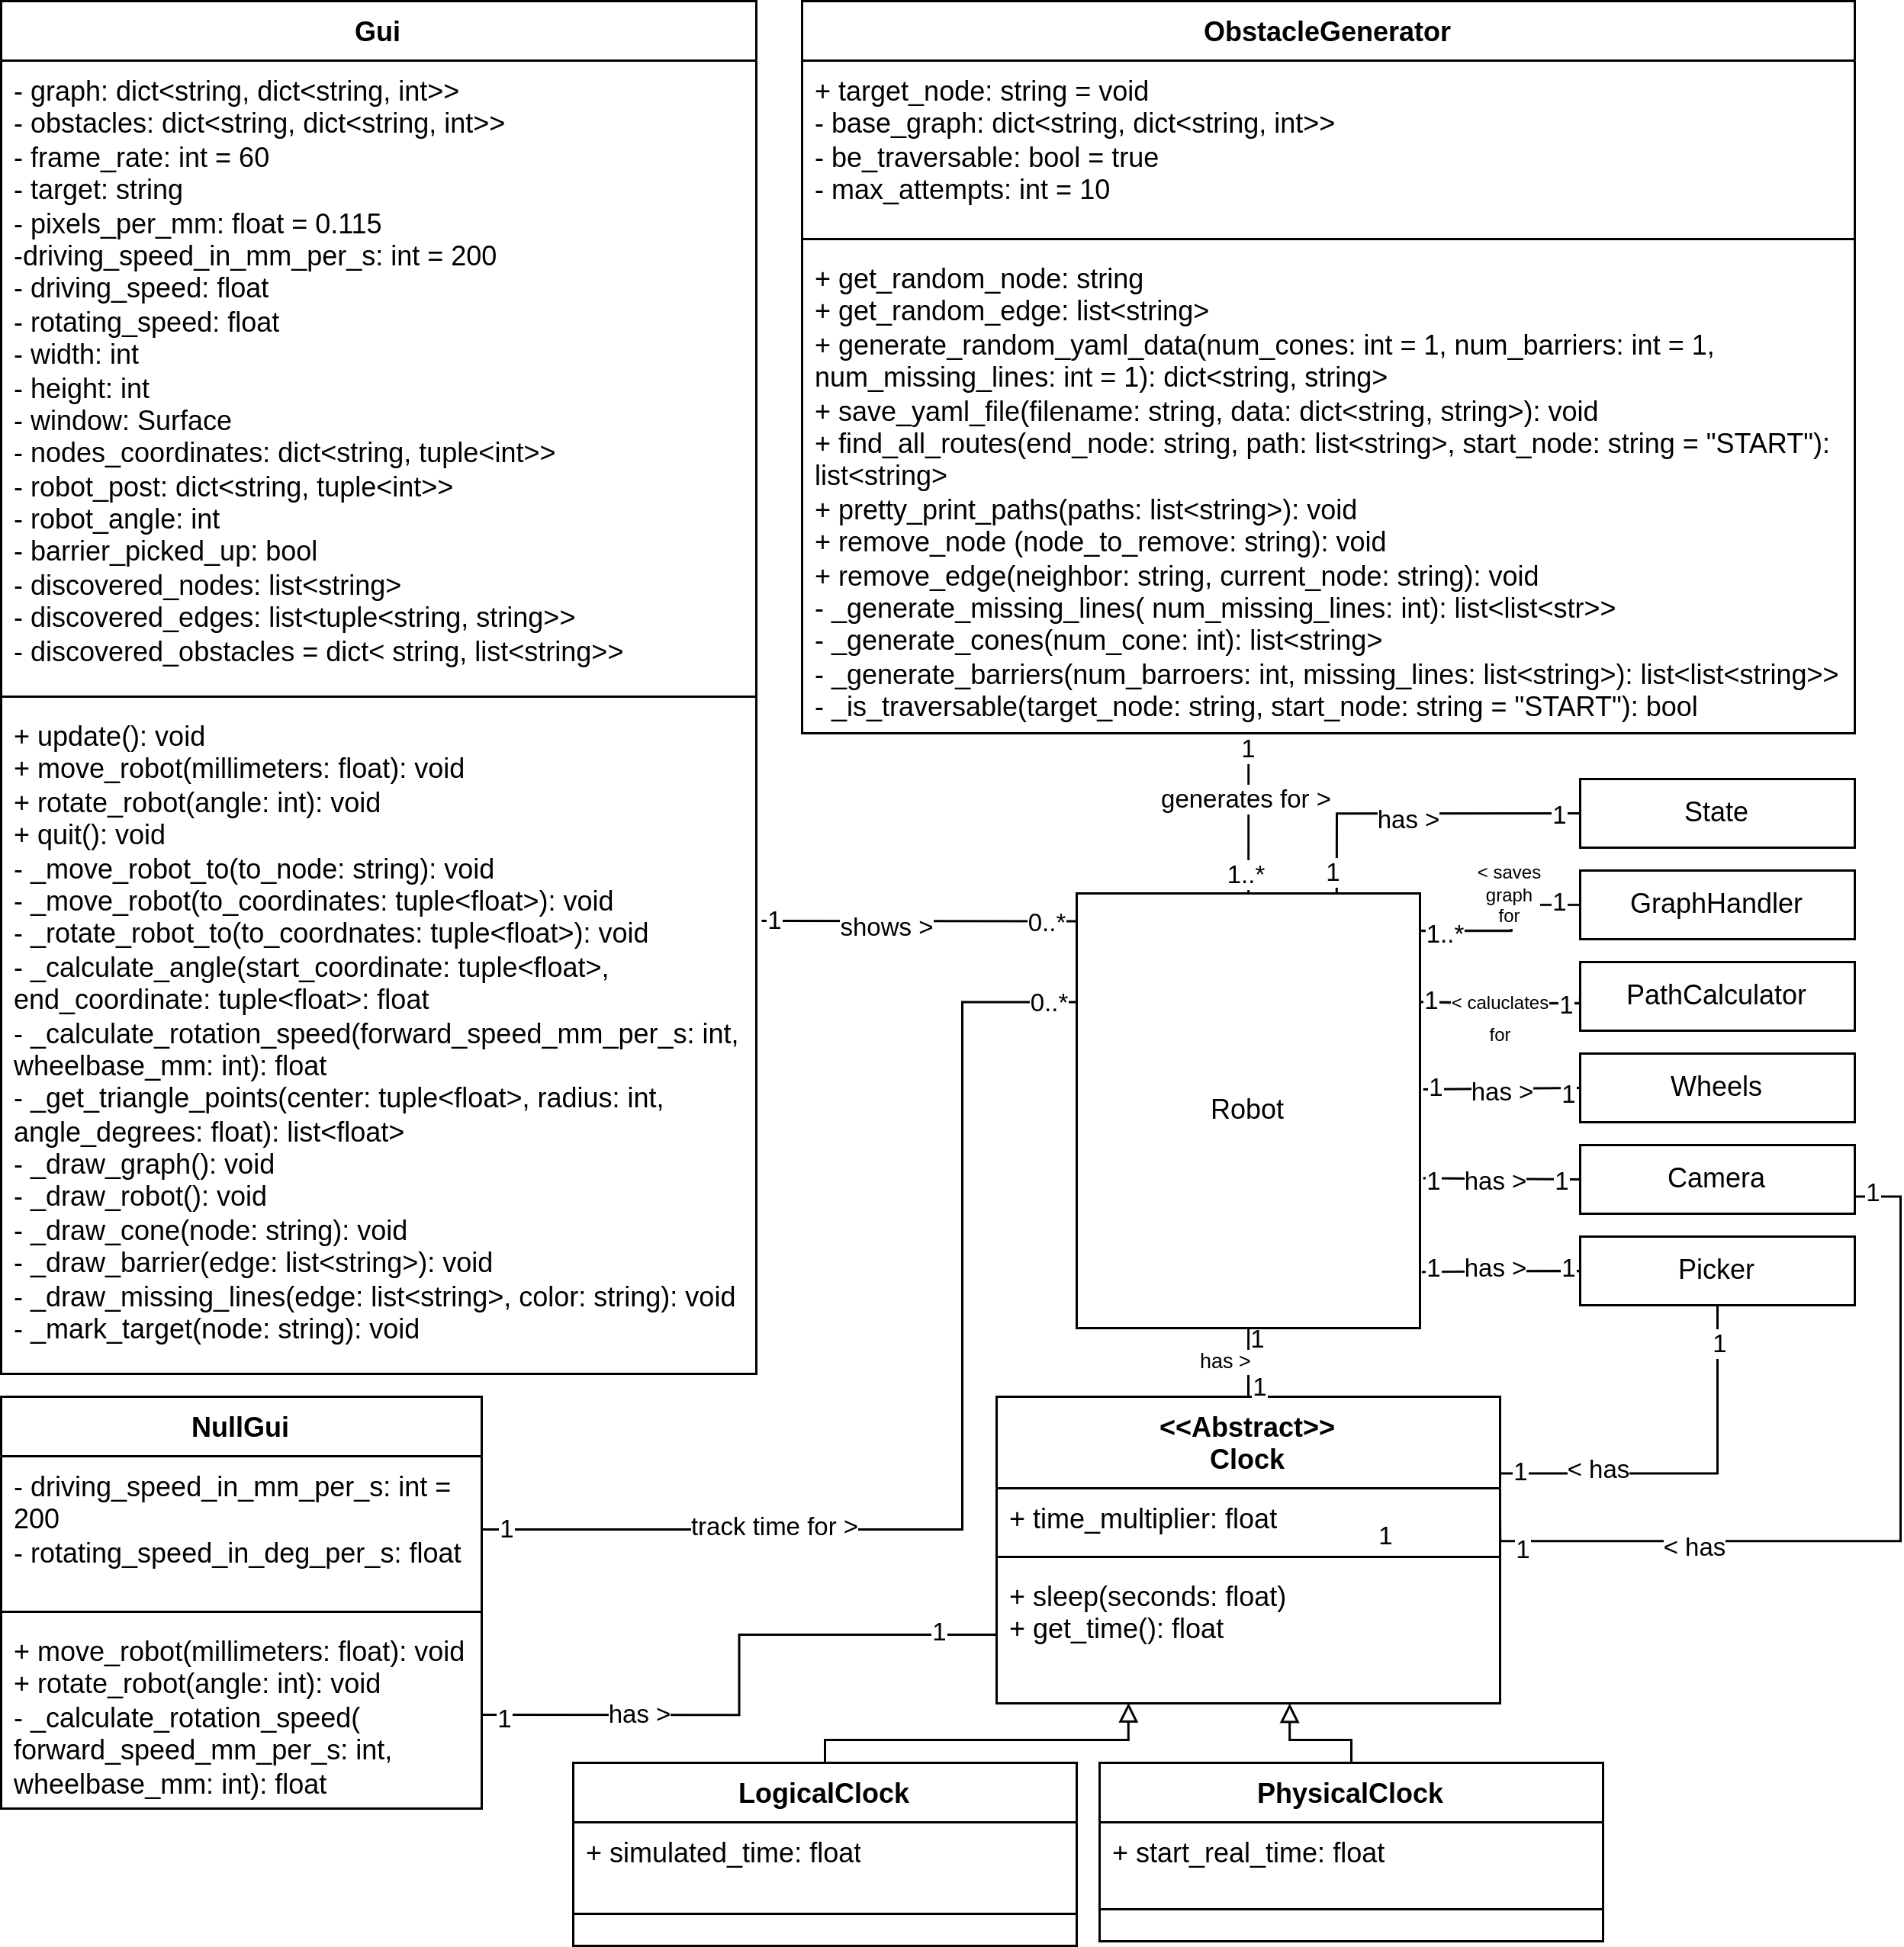
\includegraphics[width=\textwidth]{assets/informatik-prototyp/simulator/simulator-simulator-erd.png}
\caption{Simulator Klassendiagramm: Simulator Klassen}
\label{fig:simulator-classdia-sim}
\end{figure}

\subsubsection{Entwicklung}

Der erste Schritt ist es, einen Graph zu definieren. Dabei wird in \gls{yaml} der konfigurierte Graph erstellt. 
Dazu wird der vorgegebene Graph beschriftet: Jeder Knoten erhält einen Buchstaben und jede Kante ein Gewicht. Die Gewichtungen sind die Längen der Strecken in Millimeter. Diese Beschriftung wird wie in Abbildung \ref{fig:graph-yaml} gezeigt in einem \gls{yaml} File beschrieben.

\begin{figure}[H]
\centering
\begin{subfigure}{0.37\textwidth}
\centering
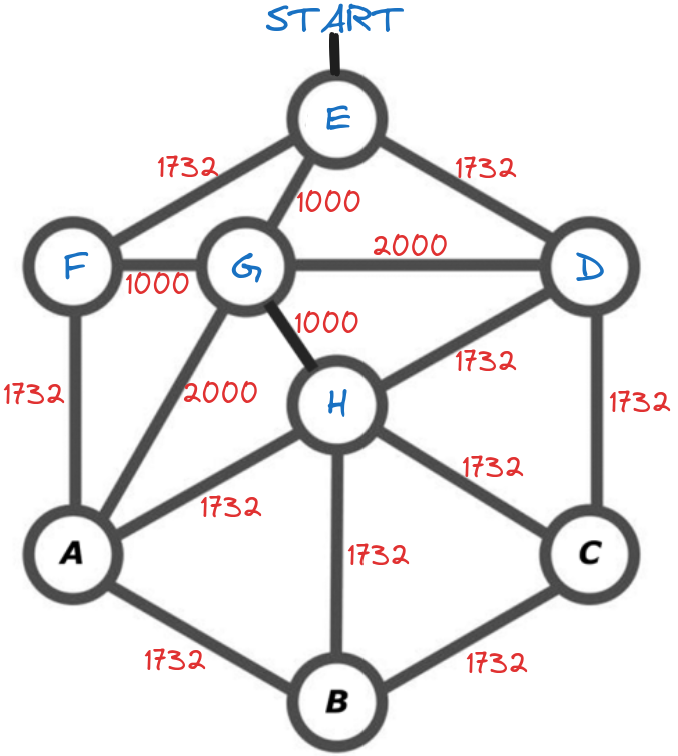
\includegraphics[width=0.95\linewidth]{img/graph_with_weighted_edges_1.png} 
\caption{Beschrifteter Graph}
\label{fig:labeled-graph}
\end{subfigure}
\begin{subfigure}{0.6\textwidth}
\begin{footnotesize}
\begin{verbatim}
START: { E: 300 }
A: { F: 1732, G: 2000, H: 1732, B: 1732 }
B: { A: 1732, H: 1732, C: 1732 }
C: { D: 1732, B: 1732, H: 1732 }
D: { E: 1732, C: 1732, H: 1732, G: 2000 }
E: { START: 300, D: 1732, G: 1000, F: 1732 }
F: { E: 1732, G: 1000, A: 1732 }
G: { E: 1000, D: 2000, H: 1000, A: 2000, F: 1000 }
H: { G: 1000, D: 1732, C: 1732, B: 1732, A: 1732 }
\end{verbatim}
\end{footnotesize}
\caption{Graph in YAML}
\label{fig:graph-yaml}
\end{subfigure}
\caption{Graph gewichten}
\label{fig:labeled-graph-and-yaml}
\end{figure}

Die Hindernisse und die fehlenden Linien sind in einem weiteren \gls{yaml} File definiert. So können diese einfach angepasst werden:

\begin{verbatim}
cone:
  - F
barrier:
  - [E, G]
missing_line:
  - [E, D]
\end{verbatim}

Der Simulator liest die beiden Dateien ein und speichert sie intern als Python Dictionaries. Ein Dictionary ist ein Datentyp, der Daten als Key-Value Paare speichert.

\textbf{Ablauf des Simulators}

Das Ziel ist es, dass der Ablauf möglichst nah an den Ablauf des Gesamtkonzeptes herankommt.
Der Programmablauf besteht aus folgenden Teilen:
\begin{enumerate}
    \item Winkel der ausgehenden Kanten vom aktuelle Knoten detektieren
    \item Nachbarsknoten auf Hindernisse prüfen
    \item Nächste Knoten berechnen
    \item Zu nächstem Knoten fahren
\end{enumerate}

Bevor der Roboter eine Knoten befährt, welcher er noch nicht kennt, überprüft dieser die Winkel der ausgehenden Kanten dieses Knoten. Im Simulator wird dies statt durch Kamerabilder, durch eine Dictionary Abfrage realisiert.
Wie beim echten Roboter detektieren wir so auch nur Kanten, die vorhanden sind und können so die fehlenden Kanten aus dem internen Graphen löschen. Die Verarbeitung der vorhandenen Winkeln wird gleich umgesetzt, wie im Gesamtkonzept Kapitel \ref{outgoing-angles} beschrieben.

Nach dem Befahren des Knotens werden alle ausgehenden Kanten überprüft. Dies geschieht durch die Drehung um die eigene Achse. Durch die Winkelmessung im vorherigen Schritt kann die optimale Drehrichtung und Reihenfolge der zu überprüfenden Nachbarsknoten berechnet werden. Der Roboter dreht sich im effizientesten Weg im Kreis und prüft alle ausgehenden Kanten und Nachbarsknoten. 
In der Simulation wird dafür das Hindernis-Dictionary auf die jeweiligen Knoten und Strecken geprüft. Falls ein Hindernis detektiert wird, reagiert der Roboter wie folgt:

\begin{itemize}
    \item Ein Pylon steht auf dem Nachbarsknoten: Dieser Knoten und alle Kanten, die dahin führen, werden im intern gespeicherten Graph-Dictionary entfernt.
    \item Eine Barriere wird auf einer ausgehenden Strecke erkannt: Die Strecke wird im intern gespeicherten Graph-Dictionary höher gewichtet. Die Höhe der neuen Gewichtung widerspiegelt sich im Verhältnis zur Zeit, der das zusätzliche Abhandeln des Objektes entspricht.
\end{itemize}

Falls noch nie eine Berechnung des kürzesten Weges durchgeführt wurde oder sich der intern gespeicherte Graph verändert hat, wird die Berechnung des kürzesten Pfades mittels \gls{dijkstra} durchgeführt. Der geplante Pfad wird gespeichert.

Danach bewegt sich der Roboter zum nächsten Knoten. Dabei wird simuliert, dass sich der Roboter zur nächsten Linie drehen soll und die Distanz zum nächsten Knoten fahren soll.


% Im Simulator sind alle Kanten eines Knotens im Uhrzeigersinn angeordnet gespeichert. Die Position (relativ zu der Strecke, von der der Roboter herkommt) der nächsten Strecke wird mit dem Ring Buffer \footnote{\url{https://en.wikipedia.org/wiki/Circular\_buffer}} zirkulär berechnet. So kann simuliert werden, dass eine Liste in einem Kreis angeordnet ist. So wird es in der richtigen Applikation möglich sein, die Kanten zu identifizieren. 

% \begin{figure}[H]
% \centering
% 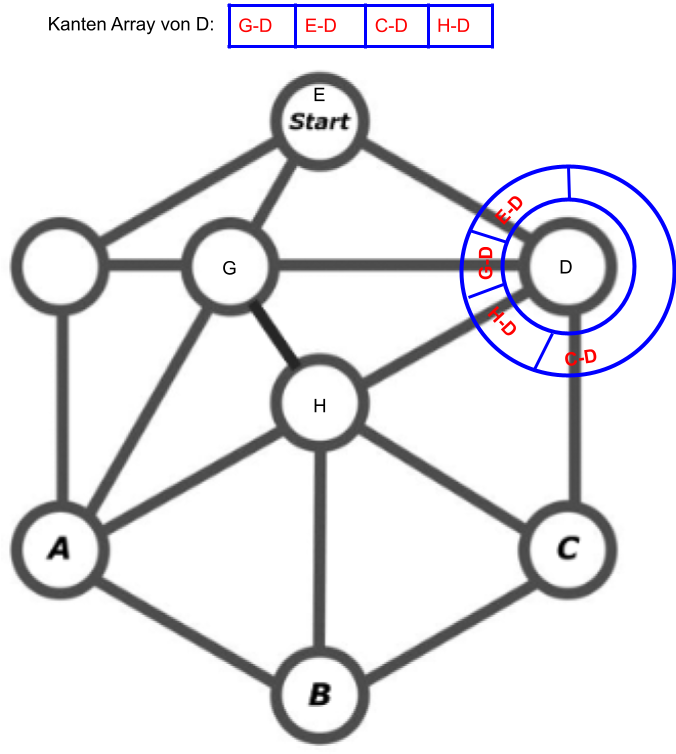
\includegraphics[width=0.5\textwidth]{assets/informatik-prototyp/simulator/ring-buffer-graph.png}
% \caption{Graph with Ring Buffer}
% \label{fig:ring-buffer-graph}
% \end{figure}

% Die Position relativ zu einer bestimmten Kante herauszufinden wird wie folgt implementiert:

% \begin{verbatim}
% edges_to_target = (target_index - start_index) % len(neighbors)
% \end{verbatim}

% Dieser Ablauf wird so lange wiederholt, bis der Zielknoten erreicht wird.
% Während des ganzen Ablaufes werden die einzelnen Klassen aufgerufen, welche die die einzelnen Roboterbauteile simulieren. In diesen befindet sich zum Teil eine Mock-Logik (zum Beispiel Hindernisse aus dem Konfigurationsfile lesen anstatt aus Bildern von der Kamera detektieren) und oft nur simple Print-Statements. Diese Print-Statements sollen die Schnittstelle zu der Elektronik simulieren.

\textbf{Trial and Error Mode}

Ein Modus \verb|BLIND_TESTING| wurde implementiert, der aktiviert wird, wenn der Roboter nicht mehr weiss, wo er sich befindet. Dieser Modus dient im realen Roboter als Risikominderung. Dabei wird der Roboter die Hindernisse und Knoten gleich erkennen, wie im normalen Modus, jedoch wird nicht der schnellste Weg berechnet. Der Roboter kennt alle ausgehenden Kanten des nächsten Knotens und die Hindernisse, die sich darauf befinden. Er wird nun jeweils ohne Berechnung die erste Kante, die nicht zu einem Pylonen führt, von links aus nehmen und so blind den Graphen traversieren, bis mit der Kamera der richtige Zielknoten erkannt wird.

Momentan ist noch nicht fest definiert, unter welchen Bedingungen zu diesem Modus gewechselt wird. Dies wird in \acrshort{pren2} festgelegt wenn Tests mit Roboterprototypen durchgeführt werden.

\textbf{Technische Aspekte}\label{technical-aspect-simulator}

Um die Abhängigkeiten zu externen Bibliotheken zu organisieren wird Poetry\footnote{\url{https://python-poetry.org/}} verwendet. Dabei werden die Bibliotheken in eine virtuelle Umgebung installiert, worin der Simulator ausgeführt wird.

\textbf{Graphical User Interface}\label{gui}

Das \acrshort{gui} wurde mit PyGame\footnote{\url{https://www.pygame.org/news}} umgesetzt. In diesem wird der Graph mit beschrifteten Knoten visualisiert. Der Roboter wird als Kreis dargestellt, an dem sich ein Dreieck befindet, dessen Spitze die Blickrichtung des Roboters angibt. Pylonen werden als orangefarbene Dreiecke, Barrieren als rote Rechtecke, und fehlende Kanten durch gestrichelte Linien visualisiert. Der Zielknoten ist mit einer roten Fahne markiert.
Ausgegraut ist alles, was der Roboter zum aktuelle Zeitpunkt noch nicht kennt, respektive noch nicht erforscht hat. Dies ist auf Abbildung \ref{fig:sim-gui} gezeigt.

\begin{figure}[H]
\centering
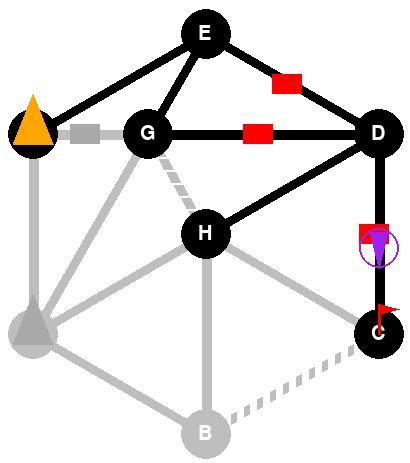
\includegraphics[width=0.5\textwidth]{assets/informatik-prototyp/simulator/sim-ui.png}
\caption{GUI des Simulators}
\label{fig:sim-gui}
\end{figure}

Das Aufheben und Absetzen der Barrieren sind mittels Farbwechsel des Roboters dargestellt.
In Abbildung \ref{fig:sim-gui-barrier-flow} ist veranschaulicht, wie eine Barriere durch den Roboter abgehandelt wird.

\begin{figure}[H]
\centering
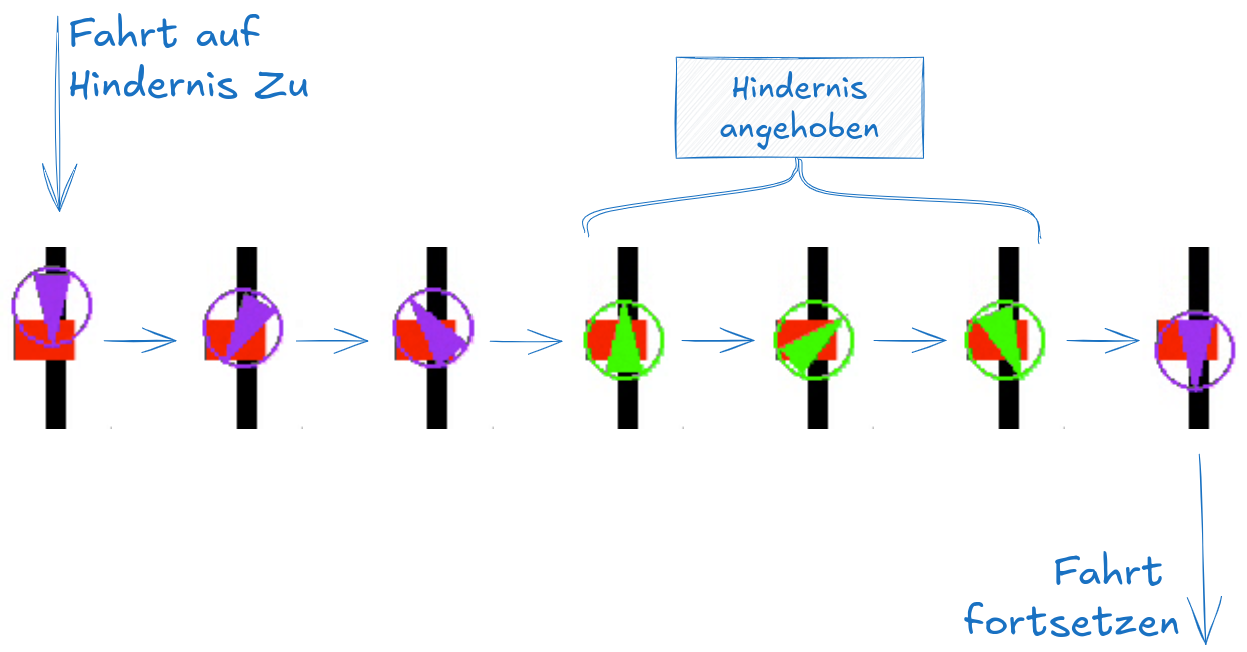
\includegraphics[width=0.75\textwidth]{assets/informatik-prototyp/simulator/sim-ui-barrier-flow.png}
\caption{GUI Barriere anheben und drehen}
\label{fig:sim-gui-barrier-flow}
\end{figure}



\subsubsection{Simulation}

In diesem Abschnitt wird erläutert wie der Simulator aufgesetzt wird, und wie dieser verwendet wird. Zusätzlich wurden automatisierte Testdurchläufe durchgeführt. Deren Ergebnisse sind anschliessend dokumentiert.

\textbf{Voraussetzungen und Installation}

Wie in Kapitel \ref{technical-aspect-simulator} erwähnt, wird unser Simulator in einer virtuellen Python Umgebung ausgeführt. Um diese Virtuelle Python Umgebung zu nutzen müssen Python Version 3.9 oder neuer und Poetry Version 1.8 oder neuer installiert sein.

Sofern dies installiert ist, kann im Grundverzeichnis des Simulators der nachfolgende Befehl ausgeführt werden, um die Abhängigkeiten zu installieren.

\begin{verbatim}
poetry install
\end{verbatim}

\textbf{Simulator ausführen}

Danach wird mit folgendem Befehl eine einfache Simulation gestartet:

\begin{verbatim}
poetry run python -m simulator
\end{verbatim}

Alle Optionen welche der Simulator bietet, können mit dem Argument \verb|--help| angezeigt werden:

\begin{footnotesize}
\begin{verbatim}
poetry run python -m simulator --help
usage: simulator [-h] [-s START_NODE] [-t {A,B,C}] [-r] [-c CONES] [-b BARRIERS] 
[-l MISSING_LINES] [--no-gui] [--speed SPEED] [--time-multiplier TIME_MULTIPLIER] 
[--simulate-time] [--verbose]

PREN1 Simulator

options:
  -h, --help                        show this help message and exit
  -s START_NODE, --start-node START_NODE
  -t {A,B,C}, --target-node {A,B,C}
  -r, --random                      Generate random obstacles
  -c, --cones CONES                 if random: Number of cones to add
  -b, --barriers BARRIERS           if random: Number of barriers to add
  -l, --missing-lines MISSING_LINES if random: Number of missing-lines to add
  --no-gui                          Run simulation without gui
  --speed SPEED                     Speed of the robot in mm/s
  --time-multiplier TIME_MULTIPLIER multiplier for all simulations
  --simulate-time                   Simulate time for task that the robot does
  --verbose                         Prints the single steps
\end{verbatim}
\end{footnotesize}

Die wichtigsten dieser Aktionen sind nachfolgend erklärt:

\begin{itemize}
    \item \verb|--random|: Ermöglicht das automatische Generieren von Hindernissen.
    \item \verb|--cones|, \verb|--barriers|, \verb|--missing-lines|: Bestimmen, wie viele Hindernisse im generierten Graph platziert werden. Standardmässig werden jeweils 2 Stück platziert.
    \item \verb|--no-gui| und \verb|--simulate-time|: Werden verwendet, um den Simulator ohne grafisches User Interface zu starten. Die Simulation wird in diesem Modus so schnell wie möglich ausgeführt. Dies ist äusserst hilfreich, wenn eine sehr grosse Anzahl an Simulationen durchgeführt werden soll.
    \item \verb|--verbose|: Ermöglicht Debugging-Ausgaben des Simulators in der Konsole.
\end{itemize}

Jede Ausführung gibt jeweils auch Informationen über den Verlauf der Simulation. Nachfolgend ein Ausschnitt einer Ausgabe:

\begin{footnotesize}
\begin{verbatim}
[...]
[2024-12-26 16:47:56,305] DRIVE 816.0MM.
[2024-12-26 16:48:00,409] DRIVE -100MM.
[2024-12-26 16:48:01,932] DRIVE 100MM.
[2024-12-26 16:48:02,451] [ET] I am now infront of my next node B. I will now check for 
    the next 1 connections.
[2024-12-26 16:48:02,451] TURN -60 DEGREES.
[2024-12-26 16:48:04,134] TAKE PIC
[2024-12-26 16:48:04,134] Planned path is ['A', 'B', 'C']
[2024-12-26 16:48:04,134] The next node considering the shortest path is node C
[2024-12-26 16:48:04,134] Moving from B to C which is 0 degrees from current direction
[2024-12-26 16:48:04,134] TURN 0 DEGREES.
[2024-12-26 16:48:04,136] DRIVE 1732MM.
[2024-12-26 16:48:12,820] DRIVE -100MM.
[2024-12-26 16:48:14,353] Expected a line from node C to D with angle 0deg
[2024-12-26 16:48:14,353] DRIVE 100MM.
Reached the target C via ['START', 'E', 'D', 'E', 'F', 'A', 'B', 'C']
traversing the graph took 84.728 seconds
\end{verbatim}
\end{footnotesize}

Bei erfolgreichem Traversieren des Graphens wird am Ende der gesamte Pfad, der genommen wurde, sowie die benötigte Zeit dafür ausgegeben.

Der Verlauf kann auch im grafischen User Interface verfolgt werden. Dabei sind die Hindernisse, welche bereits erkannt worden sind, eingefärbt. Der Pfad, der bereits bekannt ist, ist schwarz. Grau hingegen sind alle Pfade und Hindernisse welche zu dem Zeitpunkt noch unbekannt sind. Dies ist ersichtlich in Abbildung \ref{fig:simulation-run}.
Die Anzeige aktualisiert sich laufend.

\begin{figure}[H]
    \centering
    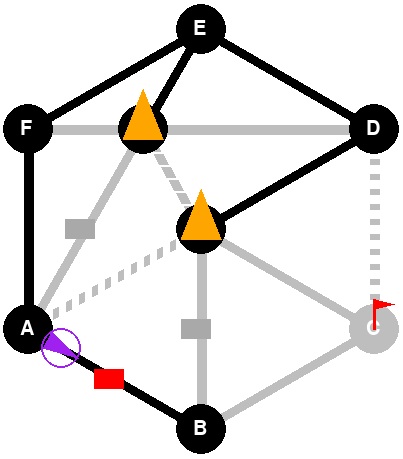
\includegraphics[width=0.5\linewidth]{assets//informatik-prototyp//simulator/simulator-run.png}
    \caption{GUI während Simulation}
    \label{fig:simulation-run}
\end{figure}

\textbf{Benchmark}

Durch das Setzen des \verb|--random| Arguments können zufällig generierte Graphen erstellt und traversiert werden.
Wenn zusätzlich \verb|--simulate-time| definiert wird, wird die Ausführungszeit ebenfalls simuliert.
Somit können fast unbegrenzt mögliche Graphen erstellt und die Traversierung mit dem Roboter in der selben Sekunde simuliert werden.

Dies wurde nun mit nachfolgenden Optionen durchgeführt:

\begin{itemize}
  \item Anzahl Pylonen: 0-6
  \item Anzahl Barrieren: 0-15
  \item Anzahl fehlende Kanten: 0-13
  \item Zielknoten: A, B oder C
\end{itemize}

Mit allen möglichen Optionen wurden so 4'215'593 verschiedene Graphen erstellt und die Traversierung dieser simuliert.
Dabei ist wichtig, dass die Traversierung des Roboters ca. 2 Minuten oder weniger dauert, egal welcher Graph mit welchen Hindernissen traversiert wird, damit die Effizienz des Roboters sichergestellt werden kann.

Nachfolgend in Abbildung \ref{fig:simulation-run-chart} sind diese Durchläufe und deren Laufzeiten in einer Grafik dargestellt. Die Simulationen sind nach Anzahl Hindernissen gruppiert. Der erste Block hatte 0 Pylonen und iterierte dabei über alle möglichen Anzahlen von Barrieren und fehlenden Linien. Der letzte Block hatte die maximale Anzahl an 5 Pylonen und iterierte ebenfalls über alle möglichen Anzahlen von Barrieren und fehlenden Linien.
Die Zahlen der Hindernisse sind im unteren Liniendiagramm ersichtlich. Das darüberliegende Liniendiagramm zeigt die dazu erreichten maximalen, minimalen und durchschnittlichen Laufzeiten.

\begin{figure}[H]
  \centering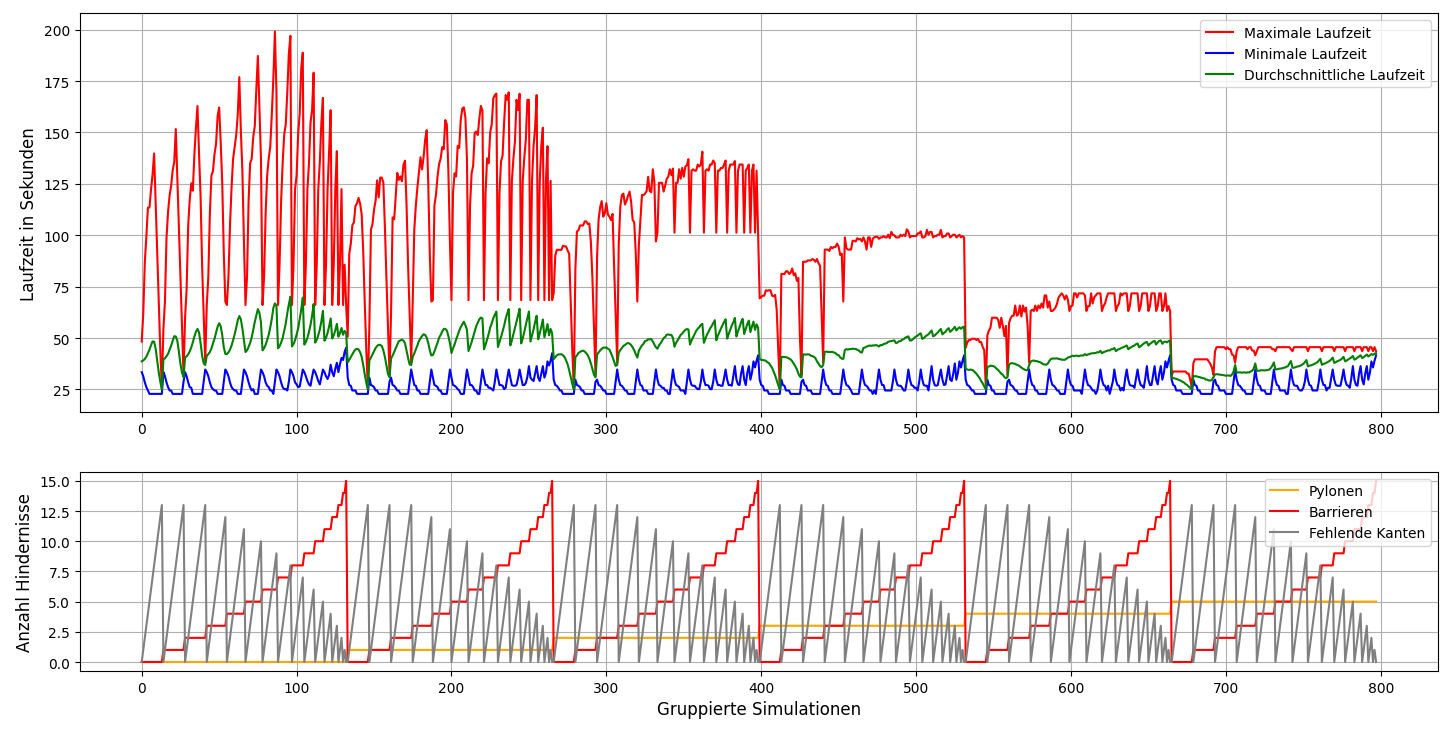
\includegraphics[width=\linewidth]{assets/informatik-prototyp/simulator/simulations_chart_sm.png}
  \caption{Simulierte Laufzeiten}
  \label{fig:simulation-run-chart}
\end{figure}

Wie zu sehen ist, braucht der Roboter im ungünstigsten Fall ungefähr 200 Sekunden für das Traversieren. Dies ist immer noch unter der geforderten Anforderung von 240 Sekunden. 
Viel interessanter ist jedoch die durchschnittliche Zeit. Diese fällt konstant unter 60 Sekunden aus.
Somit kann davon ausgegangen werden, dass der Roboter mit der aktuellen Strategie den Graphen problemlos in der geforderten Zeit erfolgreich traversieren kann.
